\documentclass[a4paper, 10pt]{article}

%% Language and font encodings
\usepackage[english]{babel}
\usepackage[utf8]{inputenc}
\usepackage[T1]{fontenc}

%% Sets page size and margins
\usepackage[a4paper,top=2.5cm,bottom=2cm,left=2.5cm,right=1.9cm]{geometry}


%% Useful packages
\usepackage{amsmath}
\usepackage{siunitx}
\usepackage{booktabs}
\usepackage{graphicx}
\usepackage[colorinlistoftodos]{todonotes}
\usepackage[colorlinks=true, allcolors=blue]{hyperref}
\usepackage{hyperref}
\usepackage{subcaption}
\usepackage{multirow}
\usepackage{arydshln}  % dashed lines
\usepackage{changepage}

\renewcommand{\arraystretch}{1.25} % for tables

\title{Your Paper}
\author{You}

\begin{document}
\maketitle
\newpage
\begin{table}[h!]
  \begin{tabular}{@{}lrrrr@{}}
    \toprule
    \multicolumn{5}{c}{\textbf{gd}} \\
    N  &   $R_t$  &  $MSE_t$ &  Epch  & T(s)\\
    \midrule
    10       &   0.06     &  0.49       &  771     & 2.64   \\
    20       &   0.31     &  0.37       &  849     & 2.82   \\
    40       &   0.32     &  0.35       &  915     & 3.58   \\
    80       &   0.49     &  0.27       &  958     & 4.12   \\
    \hdashline
    100      &   0.48     &  0.53       &  976     & 4.90   \\
    120      &   0.47     &  0.62       &  957     & 7.15   \\
    \bottomrule
  \end{tabular} 
  \hfill
  \begin{tabular}{@{}lrrrr@{}}
    \toprule
    \multicolumn{5}{c}{\textbf{gda}} \\
    N  &   $R_t$  &  $MSE_t$ &  Epch  & T(s)\\
    \midrule
    10  & 0.17    & 0.51    & 79      &  0.28   \\
    20  & 0.25    & 0.48    & 79      &  0.53   \\
    40  & 0.29    & 0.54    & 67      &  0.58   \\
    80  & 0.22    & 0.88    & 68      &  0.59   \\                 
    \hdashline
    100 & 0.20    & 0.90    & 112     &  0.51   \\
    120 & 0.21    & 1.15    & 97      &  0.47   \\
    \bottomrule
  \end{tabular} 
  \hfill
  \begin{tabular}{@{}lrrrr@{}}
    \toprule
    \multicolumn{5}{c}{\textbf{cgf}} \\
    N  &   $R_t$  &  $MSE_t$ &  Epch  & T(s)\\
    \midrule
    10  & 0.15    & 0.50    & 11      &  0.10  \\
    20  & 0.42    & 0.38    & 17      &  0.31  \\
    40  & 0.65    & 0.28    & 30      &  0.54  \\
    80  & 0.69    & 0.29    & 44      &  0.53  \\
    \hdashline
   100  & 0.68    & 0.35    & 37      &  0.59  \\
   120  & 0.60    & 0.45    & 38      &  0.76  \\
    \bottomrule
  \end{tabular} 
  \mbox{}
  \begin{tabular}{@{}lrrrr@{}}
    \toprule
    \multicolumn{5}{c}{\textbf{cgp}} \\
    N  &   $R_t$  &  $MSE_t$ &  Epch  & T(s)\\
    \midrule
    10  & 0.17    & 0.48    & 12      &  0.10  \\
    20  & 0.33    & 0.48    & 15      &  0.40  \\
    40  & 0.60    & 0.32    & 25      &  0.48  \\
    80  & 0.67    & 0.31    & 35      &  1.59  \\
    \hdashline
   100  & 0.62    & 0.38    & 40      &  0.66  \\
   120  & 0.62    & 0.44    & 32      &  0.63  \\
    \bottomrule
  \end{tabular} 
  \hfill
  \begin{tabular}{@{}lrrrr@{}}
    \toprule
    \multicolumn{5}{c}{\textbf{bfg}} \\
    N  &   $R_t$  &  $MSE_t$ &  Epch  & T(s)\\
    \midrule
    10  & 0.18    & 0.48   & 11       & 0.15  \\
    20  & 0.43    & 0.40   & 17       & 0.30  \\
    40  & 0.77    & 0.20   & 35       & 0.86  \\
    80  & 0.91    & 0.9    & 39       & 2.34  \\
    \hdashline
   100  & 0.88    & 0.12   & 47       & 2.55  \\   
   120  & 0.75    & 0.28   & 47       & 3.59  \\
    \bottomrule
  \end{tabular} 
  \hfill
  \begin{tabular}{@{}lrrrr@{}}
    \toprule
    \multicolumn{5}{c}{\textbf{lm}} \\
    N  &   $R_t$  &  $MSE_t$ &  Epch  & T(s)\\
    \midrule
    10  & 0.18    & 0.44   & 11       & 0.07  \\ 
    20  & 0.50    & 0.38   &  6       & 0.10  \\ 
    40  & 0.85    & 0.13   & 11       & 0.18  \\ 
    \textbf{80} & \textbf{.93} & \textbf{.07}  & \textbf{6} & \textbf{.31} \\
    \hdashline
   100  & 0.90    & 0.10   & 4        & 0.26  \\
   120  & 0.81    & 0.22   & 5        & 0.27  \\  
    \bottomrule
  \end{tabular} \mbox{}
  \caption{Performance of different training algorithms. Results are the
    average ones after twenty runs on the test set. \emph{N} is the
    neurons on the hidden layer. $R_t$ and $MSE_t$ 
  stand for regression R-value and for MSE on the test set, respectively. 
  Test size is 15\% of the total data. \emph{Epch} stands for epoch of 
  convergence. \emph{T(s)} is time (seconds). Best result is 
  highlighted in bold. The dotted line separates overfitted results}
  \label{tab:train_algs}
\end{table}

\begin{figure}[h]
  \begin{adjustwidth}{-1.1cm}{-1.1cm}
  \centering
  \begin{subfigure}[t]{0.3\linewidth}
    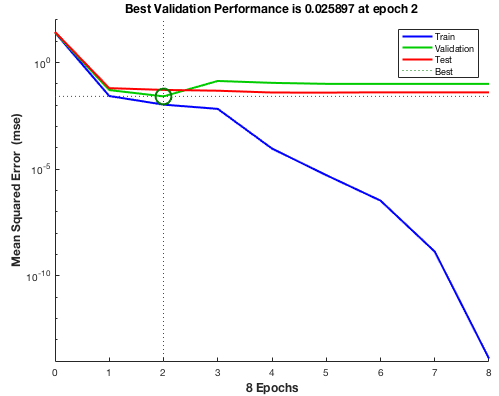
\includegraphics[width=1\linewidth]{./lab1/overfit_stop.png}
    \caption{Validation set avoids overfitting}
    \label{fig:perfect_fit}
  \end{subfigure}
  \begin{subfigure}[t]{0.3\linewidth}
    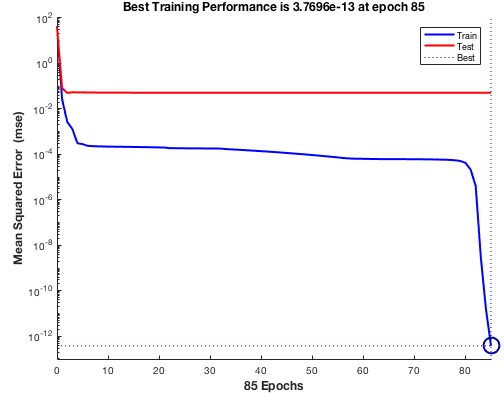
\includegraphics[width=1\linewidth]{./lab1/overfit.png}
    \caption{Overfit. 120 Neurons}
    \label{fig:overfit}
  \end{subfigure}
  \begin{subfigure}[t]{0.3\linewidth}
    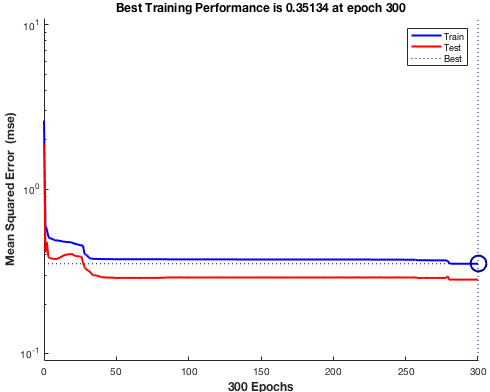
\includegraphics[width=1\linewidth]{./lab1/underfit.png}
    \caption{Underfit. 5 Neurons}
    \label{fig:underfit}
  \end{subfigure}
  \end{adjustwidth}
  \caption{Evolution of test (red), train (blue) and validation (green) set 
    MSE during training.  Left figure uses a validation set that stops befor
    e overfitting.  Otherwise, train error keeps sinking after the optima, a
    s \autoref{fig:overfit} also shows. On the right, with 5 neurons, the 
    training never converges: the net is too simple to learn the function, 
    error never decays. Test error (red) is lower than training error, it
    underfits.}
  \label{fig:validation}
\end{figure}


    \section{Algorithm comparison}
    The goal here is comparing the six algorithms for training Neural Nets on
    the Matlab toolbox. For this purpose, I have trained a net using each 
    algorithm with different number of hidden units. Then, I have evaluated
    is performance on the test set, and repeated the process twenty times. 
    \autoref{tab:train_algs} shows the results of these experiments, averaged for
    each algorithm and neuron setting. Overall, all algorithms perform best
    with 80 hidden units: nets with neurons over that threshold 
    start to overfit, since their MSE on the test set starts to decrease. 
    If there was no validation set, for 100 and 120 neurons the MSE on 
    train set would be way higher than that of test set, as
    \autoref{fig:validation} shows. On the other hand, nets with few hidden units
    do not even learn the model, and can have higher train error than test, as in
    \autoref{fig:underfit}.
    
    The best algorithm
    in terms of speed and performance is the \emph{Levenberg-Marquardt} (lm)
    algorithm: it trains the fastest, and it reaches better performance
    than the other ones under the same configurations. \emph{Gradient descent}
    is by far the worst, both in speed and accuracy. The reason is that [maybe 
    that looks for the best option/not optimized -check]



  \end{table}




\end{document}

